%
Dieses Kapitel zielt auf einen Einstieg in die N-Version Programmierung ab. In Kapitel \ref{geschichte} wird auf die Entstehungsgeschichte des Ansatzes eingegangen, woraufhin in Kapitel \ref{definition} die zugrundeliegenden Konzepte erläutert werden.
\subsection{Geschichte}\label{geschichte}
%
Design-Fehler, inkorrekte Installationen und mutwillige Angriffe zählen mit zu den Risiken in Software-Systemen. Sie können beispielsweise zu falschen oder zu spät eintreffenden Ergebnissen, Datenverlusten und als weitere Folge zu wirtschaftlichen und persönlichen Schäden führen \cite{Laprie:1995:DCC:1899254.1899261}.
Eine typische Herangehensweise der Softwareentwicklung um Fehler in Programmen zu vermeiden, besteht in der möglichst vollständigen Eliminierung von Design-Fehlern vor der Ausführung im produktiven Betrieb \cite{Avizienis:1975:FFC:800027.808469}. 
Die Idee, durch redundante Berechnungen von Ergebnissen Fehler zu erkennen und zu vermeiden, geht lange zurück. Bereits 1834 schrieb der irische Naturwissenschaftler Dionysius Lardner: \enquote{\emph{The most certain and effectual check upon errors which arise in the process of computation,	is to cause the same computations to be made by separate and independent computers; and this	check is rendered still more decisive if they make their computations by different methods.}} \cite{lardner}.
%

%
Mit der Motivation, vor allem Laufzeitfehler, die aufgrund von Design-Fehlern auftreten, zu vermeiden, erschienen Anfang der 1970er Jahre Vorschläge zum Einsatz von mehreren funktional äquivalenten Versionen des Zielprogramms \cite{methodology}.
Eine Auslegung des Konzepts der Verwendung von Redundanz zum Erzielen von fehlertoleranten Systemen wurde 1974 als \enquote{Recovery Block}-Ansatz bekannt \cite{Horning:1974:PSE:647641.733522}.
Hierbei werden Ergebnisse eines primären Blocks des Programms, wie in Abbildung \ref{graph-recovery} angedeutet, durch einen Akzeptanztest überprüft.
Falls der Akzeptanztest bei dem primären Block scheitert,wird der erste sekundäre Block ausgeführt. Dieser Prozess wird wiederholt bis ein Akzeptanztest das Ergebnis eines Blocks akzeptiert oder das System aufgrund mangelnder weiterer Blocks abbricht.
%
%
\begin{figure}[ht]
	\centering
	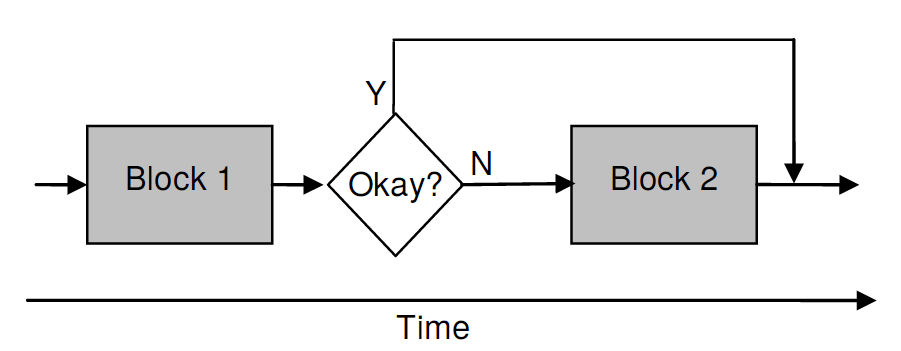
\includegraphics[width=0.8\textwidth,natwidth=901,natheight=351]{grafiken/recovery-block.png}
	\caption{Prinzip der Recovery-Blocks \cite{lucent}}
	\label{graph-recovery}
\end{figure}
%
%
Der zunächst als \enquote{redundant programming} bezeichnete Ansatz, einen systematischen Prozess zur Entwicklung von funktional equivalenten, multiversionalen Programmen zu definieren, wurde später in \enquote{N-version programming} umbennant.
Wie in Abbildung \ref{graph-n-version-single} ersichtlich, liegt der wesentliche Unterschied zum Ansatz der Recovery-Blocks darin, dass die als Versionen bezeichneten Blöcke in jedem Fall alle ausgeführt werden und statt eines Akzeptanztests ein Voting auf Basis aller Ergebnisse der verschiedenen Versionen durchgeführt wird.
Die begründende Arbeit dazu veröffentlichten Liming Chen und Algirdas Avizienis 1977 mit \enquote{\emph{N-version programming: A fault-tolerance approach to reliability of software operation}} \cite{Chen1978}.
%
%
\begin{figure}[ht]
	\centering
	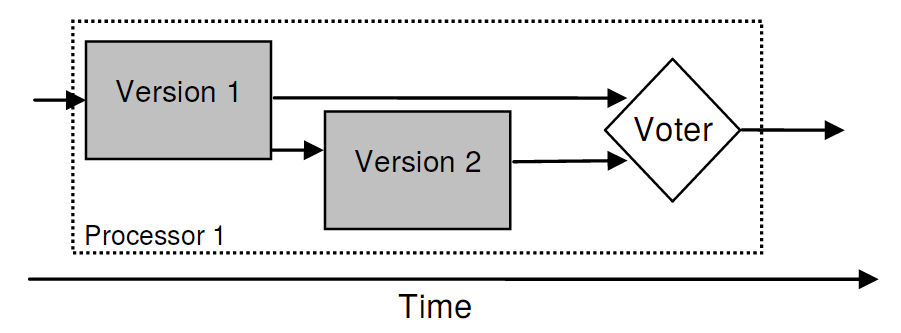
\includegraphics[width=0.8\textwidth,natwidth=901,natheight=333]{grafiken/single-thread-n-version.png}
	\caption{Voting Prinzip in der N-Version Programmierung bei Single-Threading \cite{lucent}}
	\label{graph-n-version-single}
\end{figure}
%
%
Beispiele des Einsatzes der Konzepte der N-Version Programmierung liegen vor allem mit diversen Airbus Modellen wie dem A310 in der Luftfahrt.
\subsection{Konzepte} \label{konzepte}
%
In diesem Kapitel wird zunächst der wesentliche Unterschied zwischen Single-Channel und Multi-Channel Architekturen aufgezeigt. Daraufhin wird die Definition der N-Version Programmierung vorgestellt, auf die besonderen Komponenten beim Entwurf von N-Version Programmen eingegangen und deren Funktionsweise erläutert. Abschließend werden erste Beobachtungen über die Annahmen und Limitationen des Ansatzes dargestellt.
\subsubsection{Single-Channel vs Multi-Channel} \label{channel}
%
%
Bei der mehrfachen Berechnung ($ N \geq 2 $)  eines gewünschten Ergebnisses als fundamentaler Ansatz zur Fehlertoleranz, kann zwischen den beiden Architekturen Single-Channel und Multi-Channel unterschieden werden.
Die Beschreibung der verschiedenen Konfigurationen der Architekturen kann über die Notation $(XT|YH|ZS)$ der folgenden drei Komponenten notiert werden \cite{Avizienis:1985:NAF:1314034.1314064}:
\begin{enumerate}
	\item $XT$: $X$ Anzahl an hintereinander ausgeführten Berechnungen
	\item $YH$: $Y$ eingesetzte (Hardware-)Plattformen $H$
	\item $ZS$: $Z$ eingesetzte Software-Versionen $S$
\end{enumerate}
In einer Single-Channel Architektur werden alle Versionen einer Software auf einer einzigen Plattform $(XT|1H|ZS)$ ausgeführt. In herkömmlichen Systemen kann im Falle eines erkannten Fehlers die eingesetzte Version von einem Sicherungspunkt erneut ausgeführt $(2T|1H|1S)$, oder zusätzlich eine Kopie der ursprünglich eingesetzten Version verwendet werden $(2T|1H|2S)$.
In Multi-Channel Architekturen hingegen werden $N$ Software-Versionen auf $N$ Hardware-Plattformen gleichzeitig ausgeführt $(1T|NH|NS)$.
Mit $N=4$ Versionen und Plattformen wurde diese Architektur beispielsweise im Space Shutle der NASA eingesetzt \cite{conf/ifip/Goldberg80}.
Zum Erzielen von Fehlertoleranz durch den Ansatz der mehrfachen Berechnung in Verbindung mit Multi-Channel Architekturen müssen zwei fundamentale Bedingungen erfüllt sein. Zum einen muss die Konsistenz der initialen Zustände und Eingaben aller Berechnungen gegeben sein, zum anderen muss ein zuverlässiger Vergleichsalgorithmus die einzelnen Ergebnisse vergleichen und ein finales Ergebnis bereitstellen.
Die im Folgenden beschriebenen Eigenschaften des Entwurfs von N-Version Programmen behandeln diese Bedingungen.
%
%
\subsubsection{Definition}
Chen und Avizienis definierten 1977 N-Version Programmierung wie folgt: \enquote{\emph{N-version programming is defined as the independent generation of $ N \geq 2 $ functionally equivalent programs, called \enquote{versions}, from the same initial specification}} \cite{Chen1978}.
Das grundlegende Konzept ist dabei, dass $ N \geq 2 $ Versionen eines Programms auf Basis einer gemeinsamen initialen Spezifikation entwickelt werden und deren Ergebnisse zur Laufzeit durch einen Treiber miteinander verglichen werden.
%
%
\subsubsection{Entwurf}
Für den Entwurf eines N-Version Programms werden drei besondere Komponenten vorgesehen.
(1) Vergleichsvektoren enthalten den relevanten Zustand der jeweiligen Versionen und bestehen aus den zu vergleichenden Variablen, Statusindikatoren und aufgetretenen Ereignissen.
(2) Vergleichsindikatoren enthalten den Ausgang eines Vergleichs von Vergleichsvektoren und geben an, welche nachfolgende Aktion angestoßen werden soll. 
(3) Synchronisationsmechanismen regeln den Ablauf einer Programmausführung über Signale zwischen den Versionen und dem verwaltenden Treiber. Der Treiber kann so die Versionen bei Bedarf aktivieren und Bestätigungen empfangen, falls ihre Vergleichsvektoren bereitstehen.

Die Spezifikation eines N-Version Programms sollte folgende Punkte beinhalten:
\begin{enumerate}
	\item Die zu implementierende Funktion
	\item Datenformat der Vergleichsvektoren
	\item Die Vergleichsstellen im Ablauf der Versionen, an denen die Vergleichsvektoren verglichen werden
	\item Der verwendete Vergleichsalgorithmus
	\item Die Aktionen, die auf die jeweiligen Ausgänge der Vergleiche folgen sollen
\end{enumerate}
%
Nach Möglichkeit sollen die einzelnen Versionen von unabhängigen Entwicklerteams entworfen werden und dabei weitestgehend unterschiedliche Algorithmen, Programmiersprachen und Übersetzer benutzt werden.


\subsubsection{Funktionsweise}

Auf ein Signal des Treibers hin starten die Versionen ihren Programmablauf mit identischen Eingabewerten bis sie zu einem Vergleichspunkt kommen, ihre Vergleichsvektoren bereitstellen und in einen wartenden Zustand zurückkehren.
Für $N = 2$ Versionen besteht der Vergleichsalgorithmus in einem direkten Abgleich der Vergleichsvektoren, bei $N > 2$ in einer Wahl des mehrheitlichen Ergebnisses. Falls ein oder mehrere Versionen nicht rechtzeitig ihre Vergleichsvektoren nach Aktivierung wiedergeben, können diese abgebrochen werden. Ansonsten wird ein korrektes Ergebnis aus den vorhandenen Vergleichsvektoren bestimmt. Bei numerischen Operationen können beim Vergleich Abweichungen toleriert und ein gemeinsames Ergebnis adaptiv bestimmt werden, in das alle vorhanden Ergebnisse der Versionen einfließen. 
Die zugrunde liegende Annahme, die den zusätzlichen Aufwand der verschiedenen Versionen rechtfertigen soll, besteht darin, dass unabhängige Entwicklungsprozesse signifikant die Wahrscheinlichkeit für identische Design-Fehler in zwei oder mehr Versionen senken.
Es wird angenommen, dass falls ein Fehler auftritt, er sich nicht in allen Versionen wiederfindet und durch den Vergleich der Ergebnisse ein korrektes Endergebnis erzielt wird.
%
%
\subsubsection{Beobachtungen}
Der Kern eines N-Version Programms ist die Spezifikation.
Da alle erstellten Versionen auf einer gemeinsamen Spezifikation basieren, ist ihre Korrektheit, Vollständigkeit und Eindeutigkeit der am stärksten limitierende Faktor einer effektiven Fehlervermeidung.
Jedoch argumentieren Chen und Avizienis, dass formale Korrektheitsbeweise der Spezifikationen weniger aufwändig aufgestellt werden können, als Beweise der konkreten Implementation eines Programms.
Im Vergleich zum Recovery-Block-Ansatz muss kein Akzeptanztest konzipiert werden, der ähnlich komplex wie die zu implementierende Funktion sein kann. Zudem kann bei einem Fehler in einer Version trotzdem in einem Durchlauf ein vermutlich korrektes Ergebnis erzielt werden. Allerdings muss länger auf Ergebnisse gewartet werden, falls die Versionen lediglich auf einem Prozessor arbeiten, da diese nacheinander abgearbeitet werden müssen. Diese Verzögerung kann durch den Einsatz einer Multi-Channel Architektur $(1T|NH|NS)$, welche die parallele Ausführung aller Versionen erlaubt, aufgehoben werden. Dies kann, wie in Abbildung \ref{graph-n-version-multi} angedeutet, durch  Multi-Threading oder dem Streuen von Versionen auf verschiedene Einheiten in einem verteilten System aufgehoben werden. 
%
\begin{figure}[ht]
	\centering
	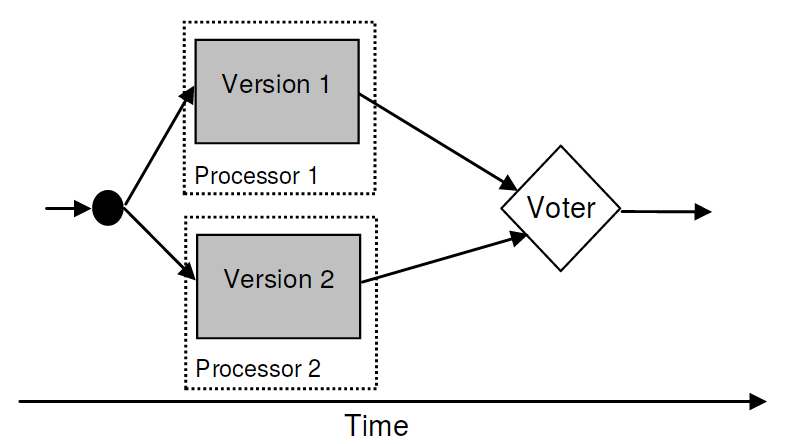
\includegraphics[width=0.8\textwidth,natwidth=901,natheight=333]{grafiken/multi-thread-n-version.png}
	\caption{Voting Prinzip in der N-Version Programmierung bei Multi-Threading \cite{lucent}}
	\label{graph-n-version-multi}
\end{figure}
%
